% This is sigproc-sp.tex -FILE FOR V2.6SP OF ACM_PROC_ARTICLE-SP.CLS
% OCTOBER 2002
%
% It is an example file showing how to use the 'acm_proc_article-sp.cls' V2.6SP
% LaTeX2e document class file for Conference Proceedings submissions.
% ----------------------------------------------------------------------------------------------------------------
% This .tex file (and associated .cls V2.6SP) *DOES NOT* produce:
%       1) The Permission Statement
%       2) The Conference (location) Info information
%       3) The Copyright Line with ACM data
%       4) Page numbering
%
%  However, both the CopyrightYear (default to 2002) and the ACM Copyright Data
% (default to X-XXXXX-XX-X/XX/XX) can still be over-ridden by whatever the author
% inserts into the source .tex file.
% e.g.
% \CopyrightYear{2003} will cause 2003 to appear in the copyright line.
% \crdata{0-12345-67-8/90/12} will cause 0-12345-67-8/90/12 to appear in the copyright line.
%
% ---------------------------------------------------------------------------------------------------------------
% It is an example which *does* use the .bib file (from which the .bbl file
% is produced).
% REMEMBER HOWEVER: After having produced the .bbl file,
% and prior to final submission,
% you need to 'insert'  your .bbl file into your source .tex file so as to provide
% ONE 'self-contained' source file.
%
% Questions regarding SIGS should be sent to
% Adrienne Griscti ---> griscti@acm.org
%
% Questions/suggestions regarding the guidelines, .tex and .cls files, etc. to
% Gerald Murray ---> murray@acm.org
%
% For tracking purposes - this is V2.6SP - OCTOBER 2002


\documentclass[12pt]{article}

\setlength{\oddsidemargin}{0in}
\setlength{\evensidemargin}{0in}
\setlength{\topmargin}{0in}
\setlength{\headheight}{0in}
\setlength{\headsep}{0in}
\setlength{\textwidth}{6in}
\setlength{\textheight}{9in}
\setlength{\parindent}{0in} 

\usepackage{graphicx} %For jpg figure inclusion
\usepackage{times} %For typeface
\usepackage{epsfig}
\usepackage{color} %For Comments
\usepackage[all]{xy}
\usepackage{float}
\usepackage{subfigure}
\usepackage{parskip}
\usepackage{float} 

%% Elena's favorite green (thanks, Fernando!)
\definecolor{ForestGreen}{RGB}{34,139,34}
% Uncomment this if you want to show work-in-progress comments
\newcommand{\comment}[1]{{\bf \tt  {#1}}}
% Uncomment this if you don't want to show comments
%\newcommand{\comment}[1]{}
\newcommand{\jcomment}[1]{\textcolor{ForestGreen}{\comment{Jeff: {#1}}}}
\newcommand{\emcomment}[1]{\textcolor{blue}{\comment{Elena: {#1}}}}
\newcommand{\scomment}[1]{\textcolor{red}{\comment{Seth: {#1}}}}
\newcommand{\todo}[1]{\textcolor{green}{\comment{To Do: {#1}}}}

%%%%%%%%% Abbreviations of commonly used Java types %%%%%%%%%%%%
\newcommand{\AL}{{\tt ArrayList}}
\newcommand{\ALI}{{\tt ArrayListInteger}}
\newcommand{\ALIP}{{\tt ArrayList<Integer>}} % Array List with Integer parameter
\newcommand{\ALS}{{\tt ArrayListString}}
\newcommand{\ALSP}{{\tt ArrayList<String>}}
\newcommand{\ALN}{{\tt ArrayListNumber}}
\newcommand{\ALT}{{\tt ArrayList<T>}}
\newcommand{\List}{{\tt List}} %%%%%%%% \L is already defined
\newcommand{\LI}{{\tt ListInteger}}
\newcommand{\LIP}{{\tt List<Integer>}}
\newcommand{\LT}{{\tt List<T>}}
\newcommand{\ABL}{{\tt AbstractList}}
\newcommand{\ABLI}{{\tt AbstractListInteger}}
\newcommand{\Obj}{{\tt Object}}
\newcommand{\Int}{{\tt Integer}}
\newcommand{\Str}{{\tt String}}
\newcommand{\Num}{{\tt Number}}
\newcommand{\LR}{{\tt ListReader}}
\newcommand{\LRI}{{\tt ListReaderInteger}}
\newcommand{\LRIP}{{\tt ListReader<Integer>}}
\newcommand{\LRT}{{\tt ListReader<T>}}
\newcommand{\CMP}{{\tt Comparable}}
\newcommand{\CMPT}{{\tt Comparable<T>}}
\newcommand{\PQ}{{\tt PriorityQueue}}
\newcommand{\OHM}{{\tt HashMap}}
\newcommand{\OHMKV}{{\tt HashMap<K,V>}}
\newcommand{\NIS}{{\tt NarrowedIS}} %%%% Note: this is not backward-compatible with past year's macros
\newcommand{\NR}{{\tt Narrowed}}
\newcommand{\Gen}{{\tt Generic}}
\newcommand{\NISC}{{\tt NarrowedISComp}}
\newcommand{\cv}{{\tt IS-contains-v}}
\newcommand{\cvi}{{\tt containsValue}}
\newcommand{\ISPI}{{\tt IS-put-inl}}
\newcommand{\ISCVI}{{\tt IS-contains-v-inl}}
\newcommand{\IICV}{{\tt II-contains-v-inl}}

\newcommand{\T}{{\tt T}} % type parameter
\newcommand{\TB}{{\tt <T>}} % type parameter with brackets
 
%%%%%%%%% R-prefixed classes and TestInteger %%%%%%%%%%%%%%%%%%%%%%%
\newcommand{\RAL}{{\tt RArrayList}}
\newcommand{\RALI}{{\tt RArrayListInteger}}
\newcommand{\RL}{{\tt RList}}
\newcommand{\TI}{{\tt TestInteger}}

%%%%%%%%% Abbreviations of commonly used methods %%%%%%%%%%%%
\newcommand{\get}{{\tt get}}
\newcommand{\set}{{\tt set}}
\newcommand{\add}{{\tt add}}
\newcommand{\getP}{{\tt get()}}
\newcommand{\setP}{{\tt set()}}
\newcommand{\addP}{{\tt add()}}
\newcommand{\equ}{{\tt equals}}
\newcommand{\tG}{{\tt testGet}}
\newcommand{\tS}{{\tt testSet}}
\newcommand{\tA}{{\tt testAdd}}

%%%%%%%%% Abbreviations of commonly used bytecode keywords %%%%%%%%%%%%
\newcommand{\invv}{{\tt invokevirtual}}
\newcommand{\invi}{{\tt invokeinterface}}
\newcommand{\cast}{{\tt checkcast}}

%%%%%%%%%%% Groups of specializations %%%%%%%%%%%%%%%
\newcommand{\Ogroup}{{\bf O}-group}
\newcommand{\ALgroup}{{\bf AL}-group}
\newcommand{\Cgroup}{{\bf C}-group}





\begin{document}
\pagestyle{plain}
%
% --- Author Metadata here ---
%\conferenceinfo{WOODSTOCK}{'97 El Paso, Texas USA}
%\setpagenumber{50}
%\CopyrightYear{2002} % Allows default copyright year (2002) to be
%over-ridden - IF NEED BE. 
%\crdata{0-12345-67-8/90/01}  % Allows default copyright data
%(X-XXXXX-XX-X/XX/XX) to be over-ridden. 
% --- End of Author Metadata ---

\title{Improving the Interoperability between Java and Clojure}
%\subtitle{[Extended Abstract \comment{DO WE NEED THIS?}]
%\titlenote{}}
%
% You need the command \numberofauthors to handle the "boxing"
% and alignment of the authors under the title, and to add
% a section for authors number 4 through n.
%
% Up to the first three authors are aligned under the title;
% use the \alignauthor commands below to handle those names
% and affiliations. Add names, affiliations, addresses for
% additional authors as the argument to \additionalauthors;
% these will be set for you without further effort on your
% part as the last section in the body of your article BEFORE
% References or any Appendices.

\author{
Stephen Adams \\
Computer Science Discipline \\
University of Minnesota Morris\\
Morris, MN 56267\\
adams601@morris.umn.edu
}

\date{}

\maketitle
\thispagestyle{empty}

\section*{\centering Abstract}

	The goal of this paper is to explore the current state of interoperability between the Clojure and Java programming languages. Java is a statically-typed Object-Oriented language, whereas Clojure is dynamic and functional. Clojure runs on the Java Virtual Machine, which allows for Clojure programs to work with Java objects and methods directly. 
	
	Clojure was designed for interoperability with Java \cite{cloj:rationale}. However, Clojure is a new language and this means that Clojure-Java interoperability is also new. Because of this the capabilities of interoperability in Clojure are not well defined. In this paper I will introduce Clojure syntax and capabilities, and the current state of Clojure-Java interop. Then I will make suggestions for expansions on how Clojure-Java interop can be improved in the future.

\newpage
\setcounter{page}{1}

\section{An Introduction to Clojure}\label{sec:intro}
	The Clojure programming language was released by Rich Hickey in 2007 \cite{wiki}. Clojure is part of the Lisp family of languages. Some brief examples of Lisp-like syntax are:
	\begin{verbatim}
	(+ 2 3)
	\end{verbatim}
	Clojure uses prefix notation. To call a function you open a new list, the first thing in this list is the function name followed by the arguments. In the above case the function "+" takes in the ints 2 and 3 and will return 5. Also:
	\begin{verbatim}
	(+ 2 3 4)
	\end{verbatim} 
	
	is a valid function call that returns 9. Clojure supports defining functions with a variable number of arguments. 
	
	Many of Clojure's data structures are the corresponding Java data structure; strings, characters, and all of the numbers are just the Java types \cite{cloj:structs}. Clojure does, however, provide its own collections. Clojure collections are each denoted by different bracket types, table~\ref{coll:table} shows which literals correspond to each collection.
	
	\begin{table}[H]
	\caption{Clojure collection literals\label{coll:table}}	
	\begin{tabular}{ | l | c | }
	\hline
	Collection Type & Literal \\ \hline
	List & (1 2 3 4) \\ \hline
	Vector & ["apple" "banana" "orange"] \\ \hline
	Hashmap & \{ :address "1234 Baker St." :City Springfield :Zip 12345 \} \\ \hline
	Set & \#\{67 2 8.8 -78 \} \\
	\hline
	\end{tabular}
	\end{table}
	
	Clojure also has a keyword datatype, keywords are used as symbolic identifiers and are denoted by a leading colon. A common example of a keyword is :import for importing other files. 
	
	\begin{verbatim}
		(ns some.Example.File
		  (:import javax.swing.JFrame))
	\end{verbatim}
	
	The above bit of code would have been placed at the beginning of a Clojure file. This declares the namespace that the following code would be run in and that the JFrame class is available. Namespaces are used to organize bits of Clojure and also define the different options that code in that namespace are given. These options include the :import keyword.
	
	Another important Lisp feature that Clojure provides is its macro support. A macro is a textual transformation. Essentially a macro expands from one piece of code to another before any evaluation happens.
	
	Clojure code is also Clojure data types. This is known as s-expressions and is common implementation of Lisp syntax. Before Clojure is compiled into JVM bytecode it is parsed into data structures by a reader \cite{wiki}. 
	
	To define new functions you use the defn macro followed by the new functions name then a vector containing the names of any arguments the function will be passed, and finally the logic of the new function. Clojure also has a special form called def that is used to store values.
	
	\begin{verbatim}
		(def myName "Stephen")
		(defn sayHello [name]
			(str "Hello " name " I hope you're having a good day!"))
	\end{verbatim}
		The above example has stored the string ``Stephen'' under the name myName. Then a function is defined that takes in a single argument and returns a string with the value of the variable inserted into it. The call:
	\begin{verbatim}
		(sayHello myName)
	\end{verbatim}
	will return the string ``Hello Stephen I hope you're having a good day!.''
	
	\subsection{Functional Programming is Clojure}
	
	Clojure functions are first class functions. This means that functions can be treated like any other objects; specifically Clojure functions can be passed to and returned from other functions, assigned to variable or stored in data structures \cite{wiki:first-class}. Some examples of these features can be found below. 
	\begin{verbatim}
		(defn square [x] 
		  (* x x))
		
		(map square [1 2 3 4 5])
	\end{verbatim}
	
	In the above example a new square function was defined and then it is passed to the built in Clojure function map. Map takes in a function and a collection and then calls the function with each of the collection's elements as the argument. Then map returns a new collection with each of the elements now modified. In the example above the map call will return the vector [1 4 9 16 25].
	
	Clojure also supports anonymous functions. 
	
	\begin{verbatim}
	(defn all-same [vect]
      (if 
        (empty? vect) true
        (every? (fn [x] (= (first vect) x)) (rest vect)) 
      )
    )
	\end{verbatim}
	
	This example function takes in a vector and checks if every element in that vector is the same. Clojure's if is a function that takes in three arguments the first is the condition which if it evaluates to true the second argument is returned otherwise the third argument is returned. The "fn" function tells the compiler that a new function is being defined within the current scope (in this case the scope is within the function all-same). First and rest are functions that just return the first element in the vector and the rest of the vector without the first element respectively. The anonymous function which was created by fn takes the first element of vect and checks if it is equal to the argument x. The outer function every? takes a function and a collection, and returns true if the function returns true when every element in the collection is passed to it. Using an anonymous function here instead of a defn outside of all-same allows for the function passed to every? to use the first element in vect which would not be available to an outside function.
	
	\subsection{The Rationale behind Clojure}
	Rich Hickey says that he wrote his own programming language because he wanted four things \cite{cloj:rationale}:
	\begin{itemize}
		\item A Lisp
		\item Functional Programming
		\item Designed for Concurrency
		\item ``symbiotic'' with an established platform.
	\end{itemize}
	
	How Clojure fulfills the first two items has been previously covered. Clojure also supports many concurrency features. Concurrency in Clojure is a large subject and is out of scope for this paper. If you are interested I would advise starting by looking at \cite{cloj:concurrency}.
	
	Clojure is implemented on the JVM; a compiler compiles Clojure code to JVM byecode. This means that Clojure code is interoperable with Java code. Because of the interoperability ever since Clojure was released it had access to the vast amount of libraries that have been written in Java. Implementation on the JVM also came with garbage collection and other memory and resource management tools, the ability to be OS agnostic, and many other features a more complete list can be found at \cite{cloj:rationale}.   

\section{Current Java Interoperability}\label{sec:bg}
	Since Clojure and Java code both compile down to JVM bytecode Clojure can call code written in Java. I will now briefly go over the primary methods for calling Java from Clojure.
	
	\subsection{The Dot Special form}
	The simplest way to call Java methods and access Java fields is with the dot(".") special form. The dot special form will first take a class member or class name then a method name and then the arguments the method takes \cite{cloj:interop}. Here are a few examples of the dot in use.
	\begin{verbatim}
	(. "fred" toUpperCase)
	;;This will return "FRED".
	(.toUpperCase "fred")
	;;This also returns "FRED".
	\end{verbatim}
	The second case will actually expand into the first call and is just a shortcut for accessing fields or methods. There are a few more shortcuts to make accessing static Java methods and fields.
	
	\begin{verbatim}
	;;Accessing a field
	(Math/PI)
	;;Returns 3.141592653589793
	;;Calling a method
	(Math/abs -2)
	;;Returns 2
	\end{verbatim}
	
	\subsection{Java Objects in Clojure}
	Static methods are only a small part of Java. Without effective ways of dealing with objects the usefulness of Java Clojure interop would be severely limited. Fortunately Clojure provides a full set of features that makes working with Java fairly easy.
	
	To construct a new object you just use the "new" special form.
	\begin{verbatim}
	(new StringBuffer "fred")
	;;Returns #<StringBuffer fred>
	\end{verbatim} 
	
	To quickly modify an object the macro doto is available. The doto first takes a call to new, then performs the rest of the supplied arguments on that object, and finally returns the resulting object.
	\begin{verbatim}
	(doto (new StringBuffer "fred") 
	  (.setCharAt 0 \F) (.append " is a nice guy!"))
	;;Returns #<StringBuffer Fred is a nice guy!>
	\end{verbatim}
	Doto is very handy for doing sequences of set methods right after you construct an object.
	
	\subsection{New Java Objects written in Clojure}
	There are problems that cannot be effectively solved without creating custom classes. In particular gui programming in swing, the primary Java gui tool, is quite difficult without the ability to extend the standard swing classes. Proxy and gen-class are the two functions provided by Clojure to implement, extend, or create Java classes. 
	
	If you just want to do object-oriented programming in Clojure you do not need to use Java interop. There is a set of functions that create new types if you don't need to extend or implement existing Java types.
	
	\subsubsection{Proxy}
	It has been said that Clojure does Java better than Java\cite{halloway:better}. I think this is most true when using proxy. It is very common when programming in Swing in particular. When creating listeners to attach to buttons or other interactive interface devices it is very common to implement many different listeners. Proxy simplifies this process by allowing you to define a single superclass with methods that will work for your interface in most circumstances; and when you need to attach a listener instead of creating an entirely new subclass use proxy to create a new class that overwrites a few methods and inherits the rest. 
	
	Proxy is a macro that takes in two vectors and then a variable number of method declarations and returns a new object. The first vector declares which Java classes the proxy object will extend and which interfaces it implements. The second vector is a list of arguments (which can be empty) to be passed to the superclass constructor. Any other arguments that are passed to proxy are method declarations \cite{cloj:interop}. 
	
	For the following proxy examples I will be using the following basic java interface:
	
	\begin{verbatim}
	public interface TestInterface {
		int square(int x);
	}
	\end{verbatim}
	This interface is in a separate interface file and is then imported into the following Clojure file.
	\begin{verbatim}
	(def test-inter 
	  (proxy [TestInterface] [] (square [x] (* x x))))
	(. test-inter square 5)
	;;Returns 25
	\end{verbatim}
	There can be more functions than just square but they have to be defined in the interface as well. Proxy cannot define new methods not declared in the interface it inherits from or its superclass.
	
	\subsubsection{Gen-class}
	Proxy is limited by what is defined in a super class or Java interface, on the other hand, gen-class is designed for implementing fully featured Java classes. Gen-class consists of a set of options which are represented as key value pairs, keys are just keywords. Gen-class currently supports fifteen different options. The examples below were taken from~\cite{kotka}:
	
	\newpage
	\begin{verbatim}
	(ns some.Example
	  (:gen-class 
	      :prefix method-))
	  
	(defn method-toString
	  [this]
	  "Hello, world!")
	  
	\end{verbatim}
	
	In the body of the file are the methods that are associated with the new type defined by gen-class. This is a fairly simple example but it gives the basic idea of how gen-class works. The only option that this class uses is the prefix option. This option defines what each method that corresponds to the class must begin with. When you want to call the method on the object you would use the following code:
	
	\begin{verbatim}
	(def aClass (new some.Example))
	;;This constructs a new instance of the object
	(.toString aClass)
	;;Returns "Hello, world!" because method-toString 
	;;has the correct prefix.
	\end{verbatim}
	
	The ``-method'' prefix is added on automatically by Clojure when the method call is made. The prefix option can also be used to define multiple classes in the same file.
	
	\begin{verbatim}
	(ns some.Example)
	
	(gen-class
	  :name  some.Example.classA
	  :prefix classA- )
	  
	(gen-class
	  :name some.Example.classB
	  :prefix classB- )
	  
	(defn classA-toString
	  [this]
	  "I'm an A.")
	  
	(defn classB-toString
	  [this]
	  "I'm an B.")
	\end{verbatim}
	
	When you call toString on one of these objects it will return the correct result depending on the type of the object in question. Only a few options were covered here, the complete gen-class specification can be found at \cite{docs:genClass} or \cite{api:genClass}. 

		
\section{Discussion and Conclusion}\label{sec:sugg}
	In the larger scheme of the Clojure language gen-class and proxy have very limited applications. Even within the ways Clojure has of defining types that generate Java classes proxy and gen-class are a minority. Figure~\ref{type:flow} displays a  flowchart for determining which form to use to define a new type.
	
	\begin{figure}[H]
	\begin{center}
	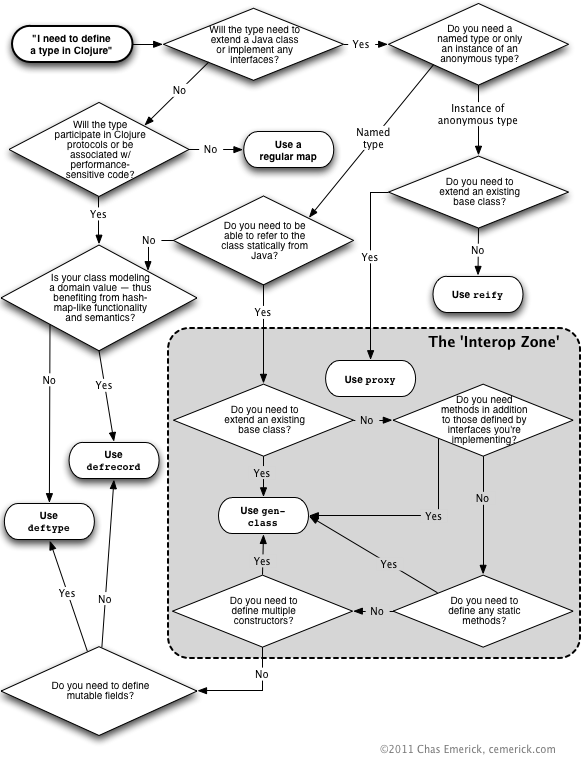
\includegraphics[scale=.55]{images/choosingtypeforms.png}
	\caption{Flowchart for choosing the correct type definition form, from \cite{choosing-types}\label{type:flow}}
	\end{center}	
	\end{figure}
	
	Gen-class and proxy are the two functions that are listed in the "interop zone" in~\ref{type:flow}. The interop zone is where Clojure's native abstractions no longer apply \cite{choosing-types}. Future work on this project may include trying to bridge the gap between other Clojure type definitions and gen-class and proxy. This may include wrapping gen-class or proxy or extending the scope of the other Clojure type definition forms so that gen-class and proxy may be depreciated. The goal would be so that to the end programmer all Clojure defined types look and feel like Clojure. 
	Additionally the information about Clojure-Java interop are scattered throughout many sources. Another goal of this project is to collect this information in one place, to include all of the relevant documentation, as well as examples and tutorials.
	
	In the forward to The Joy of Clojure\cite{joy} Steve Yegge states that it is rather surprising that a Lisp dialect has suddenly become "fashionable" again despite Clojure's lack of a killer app like Ruby has with Rails. In his contemplation on why this is he states that perhaps "the killer app for Clojure is the JVM itself. Everyone's fed up with the Java language, but understandably we don't want to abandon our investment in the Java Virtual Machine and its capabilities: the libraries, the configuration, the monitoring, and the all the other entirely valid reasons we still use it." I think that this quote simultaneously illustrates the reasons why Clojure is so compelling and why it's Java interoperability needs to be as good as possible.



%\balancecolumns

%
% The following two commands are all you need in the
% initial runs of your .tex file to
% produce the bibliography for the citations in your paper.
%\bibliographystyle{abbrv}
%\end{thebibliography}

%\bibliography{generic_types}  
% You must have a proper ".bib" file
%  and remember to run:
% latex bibtex latex latex
% to resolve all references
%
% ACM needs 'a single self-contained file'!
%
\bibliographystyle{ACM}
\bibliography{mics2012bibliography}


% That's all folks!
\end{document}

%%%%%%%%%%%%%%%%%%%%%%%%%%%%%%%%%%%%%%%%%%%%%%%%%%%%%%%%%%%%%%%%

